\documentclass[11pt,a4paper]{article}
\usepackage[utf8]{inputenc}
\usepackage[T1]{fontenc}
\usepackage{lmodern}
\usepackage{amsmath,amssymb,mathtools}
\usepackage[margin=2.2cm]{geometry}
\usepackage{microtype}
\usepackage{booktabs,array,tabularx}
\usepackage{enumitem}
\usepackage{xcolor}
\usepackage[most]{tcolorbox}
\usepackage{listings}
\usepackage{tikz}
\usetikzlibrary{arrows.meta,positioning,shapes.geometric}
\usepackage[colorlinks=true,linkcolor=blue!60!black,urlcolor=blue!60!black]{hyperref}
\usepackage{fancyhdr}
\setlength{\parindent}{0pt}
\setlength{\parskip}{6pt}
\renewcommand{\arraystretch}{1.25}
\pagestyle{fancy}
\fancyhf{}
\fancyhead[L]{\small GATE DA 2027 --- Machine Learning}
\fancyhead[R]{\small Ramu \& Somu Notes}
\fancyfoot[C]{\thepage}

\newcommand{\Oh}{\mathcal{O}}
\newcommand{\py}[1]{\texttt{#1}}

% ---------- code listings ----------
\lstdefinestyle{py}{language=Python,basicstyle=\ttfamily\small,keywordstyle=\color{blue!60!black}\bfseries,
  commentstyle=\color{green!40!black}\itshape,stringstyle=\color{red!55!black},
  backgroundcolor=\color{gray!9},frame=single,rulecolor=\color{gray!40},breaklines=true,
  showstringspaces=false,columns=fullflexible,aboveskip=4pt,belowskip=2pt,
  xleftmargin=2pt,xrightmargin=2pt}
\lstdefinestyle{out}{basicstyle=\ttfamily\small,backgroundcolor=\color{yellow!10},frame=single,
  rulecolor=\color{orange!40},breaklines=true,showstringspaces=false,columns=fullflexible,
  aboveskip=0pt,belowskip=4pt,xleftmargin=2pt,xrightmargin=2pt}
\lstset{style=py}

% ---------- boxes ----------
\newtcolorbox{story}[1][]{breakable,enhanced,colback=yellow!10,colframe=orange!80!black,
  fonttitle=\bfseries,title={Ramu \& Somu: #1},left=6pt,right=6pt,top=4pt,bottom=4pt}
\newtcolorbox{formula}[1][Key facts]{breakable,enhanced,colback=blue!5,colframe=blue!60!black,
  fonttitle=\bfseries,title={#1},left=6pt,right=6pt}
\newtcolorbox{example}[1][Worked example]{breakable,enhanced,colback=green!6,colframe=green!45!black,
  fonttitle=\bfseries,title={#1},left=6pt,right=6pt}
\newtcolorbox{trap}{breakable,enhanced,colback=red!5,colframe=red!60!black,
  fonttitle=\bfseries,title={Common GATE traps},left=6pt,right=6pt}
\newtcolorbox{intuition}{breakable,enhanced,colback=gray!8,colframe=gray!60!black,
  fonttitle=\bfseries,title={Idea in plain words},left=6pt,right=6pt}

\lstdefinestyle{sql}{style=py,language=SQL,morekeywords={IF,EXISTS,CASCADE,REFERENCES,PRIMARY,KEY,CHECK,INTERSECT,EXCEPT,LIMIT,TRIGGER,CONSTRAINT,UNIQUE,INDEX,VIEW},
  keywordstyle=\color{blue!60!black}\bfseries,commentstyle=\color{green!40!black}\itshape}
\newcommand{\sql}[1]{\texttt{#1}}
\newcommand{\key}[1]{\underline{#1}}
\newcommand{\cl}[1]{#1^{+}}
\newcommand{\fd}{\rightarrow}
\newcommand{\R}{\mathbb{R}}
\newcommand{\E}{\mathbb{E}}
\newcommand{\bx}{\boldsymbol{x}}
\newcommand{\bw}{\boldsymbol{w}}
\newcommand{\norm}[1]{\lVert #1\rVert}
\DeclareMathOperator*{\argmin}{arg\,min}
\DeclareMathOperator*{\argmax}{arg\,max}
\newcommand{\bz}{\boldsymbol{z}}
\newcommand{\bh}{\boldsymbol{h}}
\title{\Huge\bfseries GATE DA 2027\\[4pt] \Large Machine Learning\\[8pt]
\large Supervised methods, model evaluation and unsupervised methods\\
with the stories of Ramu and Somu}
\author{}
\date{}

\begin{document}
\maketitle
\thispagestyle{empty}

\begin{center}
\begin{tcolorbox}[colback=yellow!10,colframe=orange!80!black,width=0.9\textwidth,breakable]
\textbf{Ramu and Somu once more.}\\
\textbf{Ramu} asks ``but why?'' about everything. \textbf{Somu} answers with a cricket coach, a fruit market, a spam folder and a tailor.\\[4pt]
\textbf{Syllabus covered (GATE DA, Section 6):} \emph{supervised:} regression (simple, multiple, ridge) and classification (logistic regression, $k$-nearest neighbour, naive Bayes, linear discriminant analysis, support vector machines, decision trees, multi-layer perceptron/feed-forward networks); \emph{evaluation:} bias--variance trade-off, cross-validation (leave-one-out, $k$-fold); \emph{unsupervised:} clustering ($k$-means, $k$-medoids, hierarchical single/complete/average linkage) and principal component analysis.\\[4pt]
\textbf{Every number in the worked examples was computed by code} (NumPy/scikit-learn), and neural-network gradients were checked against numerical differentiation.
\end{tcolorbox}
\end{center}

\tableofcontents
\newpage

% =====================================================================
\section{The Big Picture}

\begin{story}[Learning from examples]
Ramu's cricket coach never gives a formula for a good cover drive. He shows many shots and says ``good'' or ``bad'' until Ramu's body learns the pattern. Somu: ``A machine does the same. We give it \textbf{examples} and it finds the pattern. When every example comes with an answer (a \textbf{label}), that is \textbf{supervised learning}. When there are no answers and we only ask ``what natural groups exist here?'', that is \textbf{unsupervised learning}.''
\end{story}

\begin{formula}[Vocabulary]
\begin{itemize}[noitemsep]
\item Data: $n$ examples $(\bx_i,y_i)$, $\bx_i\in\R^d$ is the \textbf{feature vector}, $y_i$ the \textbf{label/target}. Stack features in a matrix $X\in\R^{n\times d}$.
\item \textbf{Regression}: $y$ is a real number (price). \textbf{Classification}: $y$ is a category (spam/ham).
\item A \textbf{model} $f_{\bw}$ has \textbf{parameters} $\bw$ learned from data and \textbf{hyperparameters} (such as $k$, $\lambda$, tree depth) chosen by you.
\item \textbf{Loss function} $\ell(y,\hat y)$ measures one error; \textbf{training} minimises the average loss over the training set (empirical risk).
\item \textbf{Generalisation}: how well the model does on \emph{new} data. We estimate it on a held-out \textbf{test set}, never on the data used to train.
\item \textbf{Unsupervised}: only $\bx_i$ are given: clustering, dimensionality reduction (PCA).
\end{itemize}
\end{formula}

% =====================================================================
\section{Regression}

\subsection{Simple linear regression}
\begin{story}[Marks versus hours]
Ramu notes hours studied ($x$) and marks ($y$) for five friends, and wants a line to predict the marks of a sixth. Somu: ``Among all lines, pick the one with the smallest total of squared vertical gaps (\textbf{residuals}). That is \textbf{least squares}.''
\end{story}
\begin{formula}[Least-squares line $\hat y=\beta_0+\beta_1x$]
\[\beta_1=\frac{S_{xy}}{S_{xx}}=\frac{\sum(x_i-\bar x)(y_i-\bar y)}{\sum(x_i-\bar x)^2}=r\,\frac{s_y}{s_x},\qquad\beta_0=\bar y-\beta_1\bar x.\]
The line always passes through $(\bar x,\bar y)$; residuals $e_i=y_i-\hat y_i$ sum to zero.
\[\text{SSE}=\sum e_i^2,\quad\text{SST}=\sum(y_i-\bar y)^2,\quad R^2=1-\frac{\text{SSE}}{\text{SST}}\in[0,1].\]
For \emph{simple} regression $R^2=r^2$ ($r$ the correlation). $R^2$ is the fraction of the variance of $y$ explained by the model.
\end{formula}
\begin{example}[$x=1,2,3,4,5$ and $y=2,4,5,4,5$]
$\bar x=3,\ \bar y=4,\ S_{xy}=6,\ S_{xx}=10$. So $\beta_1=0.6$ and $\beta_0=4-0.6\cdot3=2.2$: $\hat y=2.2+0.6x$.\\
Residuals: $-0.8,\ 0.6,\ 1.0,\ -0.6,\ -0.2$ (sum $0$). $\text{SSE}=2.4$, $\text{SST}=6$, $R^2=1-\frac{2.4}{6}=\mathbf{0.6}$, $r=\sqrt{0.6}=0.7746$.\\
Prediction at $x=6$: $2.2+3.6=5.8$. Errors: MSE $=2.4/5=0.48$, RMSE $=0.6928$, MAE $=0.64$.
\end{example}

\subsection{Multiple linear regression and the normal equation}
\begin{formula}[Matrix form]
With $X\in\R^{n\times(d+1)}$ (first column all ones for the intercept), $\hat y=X\bw$. Minimising $\norm{y-X\bw}^2$ gives the \textbf{normal equations}
\[X^{\top}X\,\hat{\bw}=X^{\top}y\quad\Longrightarrow\quad\hat{\bw}=(X^{\top}X)^{-1}X^{\top}y.\]
Requires $X^\top X$ invertible (columns linearly independent: no perfect multicollinearity, $n\ge d+1$). Geometrically $X\hat{\bw}$ is the \emph{projection} of $y$ onto the column space of $X$, so the residual is orthogonal to every column: $X^\top(y-X\hat{\bw})=0$.\\
\textbf{Gradient descent} alternative: $\bw\leftarrow\bw-\eta\,\frac2n X^\top(X\bw-y)$. Example: data $(1,2),(2,4)$, model $\hat y=wx$, $w_0=0$: gradient of MSE $=\frac22\bigl[(-2)(1)+(-4)(2)\bigr]=-10$; with $\eta=0.1$, $w_1=1.0$ (the true $w=2$ is approached step by step).
\end{formula}
\begin{example}[Four points, two features]
$X=\begin{pmatrix}1&1&2\\1&2&1\\1&3&4\\1&4&3\end{pmatrix}$, $y=(6,6,14,13)^\top$, $X^\top X=\begin{pmatrix}4&10&10\\10&30&28\\10&28&30\end{pmatrix}$. Solving gives $\hat{\bw}=\bigl(\tfrac38,\ \tfrac{13}{8},\ \tfrac{17}{8}\bigr)$.
\end{example}

\subsection{Ridge regression (L2 regularisation)}
\begin{story}[Taming a wild line]
With many features and few examples, least squares can chase noise and produce huge weights. Somu adds a \emph{penalty on big weights}: ``You may fit the data, but every unit of weight costs you $\lambda$.'' This shrinks the weights toward zero.
\end{story}
\begin{formula}[Ridge]
\[\hat{\bw}_{\text{ridge}}=\argmin_{\bw}\ \norm{y-X\bw}^2+\lambda\norm{\bw}^2=(X^\top X+\lambda I)^{-1}X^\top y.\]
$\lambda=0$: ordinary least squares. $\lambda\to\infty$: weights $\to0$. Adding $\lambda I$ makes $X^\top X+\lambda I$ \emph{always invertible}, curing multicollinearity. The intercept is usually not penalised. Larger $\lambda$ $\Rightarrow$ more bias, less variance. \textbf{Lasso} uses $\lambda\norm{\bw}_1$ instead and drives some weights \emph{exactly} to zero (feature selection). Choose $\lambda$ by cross-validation.
\end{formula}
\begin{example}[Ridge on the marks data: slope $=\dfrac{S_{xy}}{S_{xx}+\lambda}$]
\begin{center}
\begin{tabular}{c|cccc}
$\lambda$ & 0 & 1 & 5 & 100\\\midrule
slope $\beta_1$ & 0.6000 & 0.5455 & 0.4000 & 0.0545\\
intercept $\beta_0$ & 2.2000 & 2.3636 & 2.8000 & 3.8364
\end{tabular}
\end{center}
As $\lambda$ grows the slope shrinks toward $0$ and the intercept toward $\bar y=4$.
\end{example}
\begin{trap}
(1) $R^2$ never decreases when you add features (use adjusted $R^2$ or test data). (2) Do not penalise the intercept. (3) Standardise features before ridge/lasso/kNN/SVM, since the penalty depends on scale. (4) $(X^\top X)^{-1}$ fails when features are collinear. (5) A high $R^2$ on training data does not mean a good model.
\end{trap}

% =====================================================================
\section{Classification}

\subsection{Logistic regression}
\begin{story}[A probability, not a number]
Ramu wants to predict ``will it rain?'' A line can output $-3$ or $7$, which is silly for a probability. Somu squeezes any number into $(0,1)$ with the \textbf{sigmoid} $\sigma(z)=\frac{1}{1+e^{-z}}$, and says ``rain'' when the probability exceeds $\frac12$.
\end{story}
\begin{formula}[Model and loss]
\[p(y=1\mid\bx)=\sigma(\bw^\top\bx+b),\qquad\sigma'(z)=\sigma(z)(1-\sigma(z)).\]
Log-odds are linear: $\ln\frac{p}{1-p}=\bw^\top\bx+b$, so the \textbf{decision boundary} $\bw^\top\bx+b=0$ (where $p=\frac12$) is a \emph{hyperplane}: logistic regression is a linear classifier. Fit by minimising the \textbf{cross-entropy (log) loss}
\[\ell=-\bigl[y\ln p+(1-y)\ln(1-p)\bigr],\qquad\frac{\partial\ell}{\partial\bw}=(p-y)\,\bx,\quad\frac{\partial\ell}{\partial b}=p-y.\]
The loss is convex, so gradient descent reaches the global minimum. For $K$ classes use \textbf{softmax}: $p_k=\frac{e^{z_k}}{\sum_je^{z_j}}$.
\end{formula}
\begin{example}[One example, one gradient step]
$\bw=(0.5,-0.25)$, $b=0.5$, $\bx=(2,4)$, $y=1$. Then $z=1-1+0.5=0.5$, $p=\sigma(0.5)=\mathbf{0.6225}$. Loss $=-\ln0.6225=0.4741$ (if the label were $0$, loss $=0.9741$). Gradient: $(p-1)\bx=(-0.755,-1.510)$, $\partial b=-0.3775$. With $\eta=0.1$: $\bw\leftarrow(0.5755,-0.0990)$, $b\leftarrow0.5378$ and the new probability is $0.7846$: the model is now more confident in the right class.\\
Useful values: $\sigma(0)=0.5$, $\sigma(2)=0.8808$, $\sigma(-2)=0.1192$, $\sigma(1)=0.7311$. Softmax of $(2,1,0.1)$ is $(0.659,0.242,0.099)$.
\end{example}

\subsection{$k$-nearest neighbours (kNN)}
\begin{story}[Ask the neighbours]
A new family moves in. Somu: ``To guess their cricket team, ask the $k$ closest houses and go with the majority.'' No training at all; all work happens at prediction time (a \textbf{lazy learner}).
\end{story}
\begin{formula}[kNN]
Classify $\bx$ by the majority label among its $k$ nearest training points (distance: Euclidean $\sqrt{\sum(x_j-z_j)^2}$, Manhattan $\sum|x_j-z_j|$, or other). For regression: average of the $k$ neighbours' values. \textbf{Small $k$}: flexible, low bias, high variance (overfits; $k=1$ gives zero training error). \textbf{Large $k$}: smooth, high bias (as $k=n$ it predicts the global majority). Features must be \textbf{scaled}. Prediction cost $O(nd)$ per query; it suffers in high dimensions (curse of dimensionality).
\end{formula}
\begin{example}[Query $(4,4)$]
Training points: A: $(1,1),(2,1),(2,3)$; B: $(6,5),(7,7),(8,6)$. Euclidean distances to $(4,4)$: $4.24,\ 3.61,\ 2.24,\ 2.24,\ 4.24,\ 4.47$. The $3$ nearest are $(2,3){:}A$ and $(6,5){:}B$ (both $2.24$) and $(2,1){:}A$ ($3.61$): two A against one B, so $k=3\Rightarrow$ \textbf{A}. (With $k=1$ there is a tie, which is why $k$ is usually odd.) Manhattan distances ($6,5,3,3,6,6$) give the same three neighbours.
\end{example}

\subsection{Naive Bayes}
\begin{story}[Spam by counting words]
Somu counts: of the spam emails, how many contain ``free'', how many ``win''? For a new email he multiplies these chances, pretending the words appear \emph{independently} once you know the class. That is ``naive'' but works surprisingly well.
\end{story}
\begin{formula}[Naive Bayes classifier]
By Bayes' rule $P(C\mid\bx)\propto P(C)\prod_{j=1}^dP(x_j\mid C)$ (conditional independence of features given the class). Predict $\hat C=\argmax_CP(C)\prod_jP(x_j\mid C)$. Probabilities are estimated by counting; \textbf{Laplace smoothing} fixes the zero-frequency problem: $P(x_j=v\mid C)=\dfrac{\text{count}+1}{N_C+V}$ ($V$ = number of values the feature can take). For continuous features use a Gaussian per class (mean and variance). Training is one pass over the data.
\end{formula}
\begin{example}[Six emails]
Spam: $(\text{free},\text{win})=(1,1),(1,0),(0,1)$; ham: $(0,0),(1,0),(0,0)$. New email $(1,1)$. Priors $\frac12,\frac12$.\\
\emph{Without smoothing:} spam $=\frac12\cdot\frac23\cdot\frac23=0.2222$; ham $=\frac12\cdot\frac13\cdot0=0$ (no ham email had ``win'': a single zero kills the product).\\
\emph{Laplace ($V=2$):} spam $=\frac12\cdot\frac35\cdot\frac35=0.18$; ham $=\frac12\cdot\frac25\cdot\frac15=0.04$. Posterior $P(\text{spam})=\frac{0.18}{0.18+0.04}=\mathbf{0.818}$.
\end{example}

\subsection{Linear discriminant analysis (LDA)}
\begin{formula}[LDA]
Assume each class is Gaussian with its own mean $\mu_k$ but a \textbf{shared covariance} $\Sigma$. The Bayes-optimal rule then has linear discriminants
\[\delta_k(\bx)=\bx^\top\Sigma^{-1}\mu_k-\tfrac12\mu_k^\top\Sigma^{-1}\mu_k+\ln\pi_k,\qquad\hat C=\argmax_k\delta_k(\bx),\]
with priors $\pi_k$. The boundary is linear. (With \emph{different} covariances you get quadratic boundaries: QDA.) \textbf{Fisher's view:} project onto the direction $\bw\propto\Sigma^{-1}(\mu_1-\mu_2)$ that maximises between-class separation relative to within-class scatter.\\
\textbf{One dimension, two classes:} boundary $x^*=\frac{\mu_1+\mu_2}{2}-\frac{\sigma^2\ln(\pi_1/\pi_2)}{\mu_1-\mu_2}$.
\end{formula}
\begin{example}[$\mu_1=2,\ \mu_2=6,\ \sigma^2=4$]
Equal priors: $x^*=\frac{2+6}{2}=4$ (the midpoint). Priors $\pi_1=0.7,\pi_2=0.3$: $x^*=4-\frac{4\ln(7/3)}{-4}=4+0.847=\mathbf{4.847}$: the boundary moves \emph{toward} the rarer class $2$, because class $1$ is a priori more likely.
\end{example}

\subsection{Evaluating a classifier}
\begin{formula}[Confusion matrix metrics]
\begin{center}
\begin{tabular}{l|cc}
& predicted $+$ & predicted $-$\\\midrule
actual $+$ & TP & FN\\
actual $-$ & FP & TN
\end{tabular}
\end{center}
Accuracy $=\frac{TP+TN}{N}$; precision $=\frac{TP}{TP+FP}$; recall (sensitivity, TPR) $=\frac{TP}{TP+FN}$; specificity $=\frac{TN}{TN+FP}$; FPR $=1-$specificity; $F_1=\frac{2PR}{P+R}$ (harmonic mean). Example: $TP=40,FP=10,FN=20,TN=30$: accuracy $0.70$, precision $0.80$, recall $0.667$, specificity $0.75$, $F_1=0.727$. The \textbf{ROC curve} plots TPR against FPR as the threshold varies; \textbf{AUC} (area under it) is $0.5$ for random guessing and $1$ for perfect ranking. With imbalanced classes accuracy misleads: a model that always says ``no'' on a $99\%$-negative dataset gets $99\%$ accuracy and $0$ recall.
\end{formula}
\begin{trap}
(1) Logistic ``regression'' is a classifier. (2) Naive Bayes needs smoothing for unseen feature values. (3) kNN has no training phase but costly prediction. (4) LDA assumes equal covariances; QDA does not. (5) Precision and recall trade off as the threshold moves. (6) Standardise features for distance-based methods.
\end{trap}
% =====================================================================
\section{Decision Trees}

\begin{story}[Twenty questions]
Ramu thinks of an animal and Somu asks yes/no questions. A good player first asks the question that cuts the possibilities most evenly (``Does it live in water?''), not a silly one (``Is it a dog called Moti?''). A \textbf{decision tree} is a flowchart of such questions: each internal node tests a feature, each branch is an answer, each leaf gives a class. Learning means choosing, node by node, the \emph{most informative} question.
\end{story}

\begin{formula}[Impurity measures]
For a node with class proportions $p_1,\dots,p_K$:
\begin{itemize}[noitemsep]
\item \textbf{Entropy} $H=-\sum_kp_k\log_2p_k$ (bits). $H=0$ for a pure node; $H=\log_2K$ at most (for two classes, $1$ bit at $50/50$). Example: $(1,3)\to0.8113$.
\item \textbf{Gini index} $G=1-\sum_kp_k^2$ (two classes: max $0.5$).
\item \textbf{Information gain} of splitting on attribute $A$: $\text{IG}=H(S)-\sum_{v}\frac{|S_v|}{|S|}H(S_v)$ (ID3 picks the maximum).
\item \textbf{Gain ratio} (C4.5) $=\text{IG}/\text{SplitInfo}$, with $\text{SplitInfo}=-\sum\frac{|S_v|}{|S|}\log_2\frac{|S_v|}{|S|}$; it penalises attributes with many values. CART uses Gini (binary splits).
\item \textbf{Regression trees}: leaf predicts the mean; split to maximise reduction in variance (SSE).
\end{itemize}
\end{formula}

\begin{example}[Classic weather data: 14 days, $9$ ``play'' and $5$ ``no play''; split on Outlook]
Outlook: sunny $(2,3)$, overcast $(4,0)$, rain $(3,2)$ (yes, no).
\begin{itemize}[noitemsep]
\item $H(S)=-\frac9{14}\log_2\frac9{14}-\frac5{14}\log_2\frac5{14}=\mathbf{0.940}$; Gini$(S)=1-(\frac9{14})^2-(\frac5{14})^2=0.459$.
\item $H(\text{sunny})=0.971$, $H(\text{overcast})=0$, $H(\text{rain})=0.971$.
\item Remainder $=\frac5{14}(0.971)+\frac4{14}(0)+\frac5{14}(0.971)=0.694$, so $\text{IG}(\text{Outlook})=0.940-0.694=\mathbf{0.247}$.
\item Weighted Gini after the split $=\frac5{14}(0.48)+0+\frac5{14}(0.48)=0.343$ (down from $0.459$).
\item SplitInfo $=1.577$, gain ratio $=0.247/1.577=0.156$.
\end{itemize}
The overcast branch is already pure: it becomes a leaf ``play''.
\end{example}
\begin{formula}[Growing and controlling a tree]
Greedy, top-down, recursive: pick the best split, partition, recurse; stop when a node is pure, no features remain, or a depth/size limit is reached. A fully grown tree memorises the training set (\textbf{overfitting}: low bias, high variance). Remedies: \textbf{pre-pruning} (max depth, minimum samples, minimum gain), \textbf{post-pruning} (grow, then cut back using validation data), and ensembles (random forests average many trees; boosting adds trees sequentially). Trees handle mixed feature types, need no scaling, are easy to interpret, but are unstable (small data changes change the tree) and produce axis-parallel boundaries.
\end{formula}
\begin{trap}
(1) Information gain favours attributes with many values (hence gain ratio). (2) Entropy uses $\log_2$ (bits); with natural logs the values change by a constant factor. (3) $0\log0=0$. (4) A tree can always reach $100\%$ training accuracy if no two identical inputs have different labels. (5) Do not confuse the weighted impurity \emph{after} the split with the gain.
\end{trap}

% =====================================================================
\section{Support Vector Machines (SVM)}

\begin{story}[The widest road]
Two villages, red on the left and blue on the right. Somu must build a straight road between them. ``Many roads separate the villages. The safest is the \emph{widest}, the one that keeps the greatest clearance from the nearest house on each side.'' The nearest houses are the \textbf{support vectors}: they alone hold the road in place. Move any other house and the road stays; move a support vector and the road shifts.
\end{story}

\begin{center}
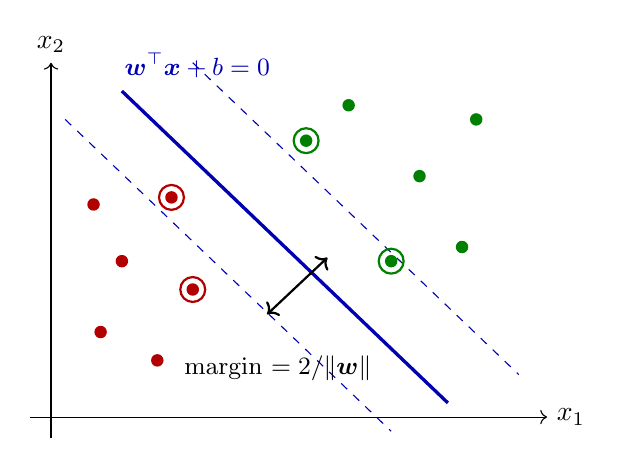
\begin{tikzpicture}[scale=0.9]
\draw[->] (-0.3,0)--(7,0) node[right]{$x_1$}; \draw[->] (0,-0.3)--(0,5) node[above]{$x_2$};
\draw[very thick,blue!70!black] (1,4.6)--(5.6,0.2); \node[blue!70!black,anchor=south west] at (0.9,4.65) {\small $\bw^\top\bx+b=0$};
\draw[dashed,blue!70!black] (0.2,4.2)--(4.8,-0.2); \draw[dashed,blue!70!black] (2,5)--(6.6,0.6);
\foreach \p in {(0.7,1.2),(1.5,0.8),(1.0,2.2),(2.0,1.8),(0.6,3.0),(1.7,3.1)} \fill[red!70!black] \p circle (2.5pt);
\foreach \p in {(4.2,4.4),(5.2,3.4),(4.8,2.2),(6.0,4.2),(3.6,3.9),(5.8,2.4)} \fill[green!50!black] \p circle (2.5pt);
\draw[red!70!black,thick] (2.0,1.8) circle (5pt); \draw[red!70!black,thick] (1.7,3.1) circle (5pt);
\draw[green!50!black,thick] (3.6,3.9) circle (5pt); \draw[green!50!black,thick] (4.8,2.2) circle (5pt);
\draw[<->,thick] (3.05,1.45)--(3.9,2.25); \node[anchor=north,align=center] at (3.2,1.0) {\small margin $=2/\norm{\bw}$};
\end{tikzpicture}
\end{center}
\begin{formula}[Hard-margin SVM]
Labels $y_i\in\{-1,+1\}$. Require every point on the correct side with clearance:
\[\min_{\bw,b}\ \tfrac12\norm{\bw}^2\quad\text{subject to}\quad y_i(\bw^\top\bx_i+b)\ge1\ \ \forall i.\]
The two margin lines are $\bw^\top\bx+b=\pm1$; the distance between them (the \textbf{margin}) is $\dfrac{2}{\norm{\bw}}$, so maximising the margin $=$ minimising $\norm{\bw}^2$. Points with $y_i(\bw^\top\bx_i+b)=1$ are the \textbf{support vectors}. Predict $\operatorname{sign}(\bw^\top\bx+b)$.\\
\textbf{Dual form:} $\bw=\sum_i\alpha_iy_i\bx_i$ with $\alpha_i\ge0$, $\sum_i\alpha_iy_i=0$, and $\alpha_i>0$ \emph{only} for support vectors. Predictions use only dot products $\bx_i^\top\bx$, which makes the kernel trick possible.
\end{formula}
\begin{formula}[Soft margin and kernels]
Real data overlap, so allow \textbf{slack} $\xi_i\ge0$: minimise $\tfrac12\norm{\bw}^2+C\sum_i\xi_i$ subject to $y_i(\bw^\top\bx_i+b)\ge1-\xi_i$. Equivalent to the \textbf{hinge loss} $\max(0,\,1-y_i(\bw^\top\bx_i+b))$ plus an L2 penalty. \textbf{$C$ large}: few violations, narrow margin (low bias, high variance, risk of overfitting); \textbf{$C$ small}: wide margin, more violations (more bias, less variance).\\
\textbf{Kernel trick:} replace $\bx_i^\top\bx_j$ by $K(\bx_i,\bx_j)=\phi(\bx_i)^\top\phi(\bx_j)$ to get a non-linear boundary without computing $\phi$. Common kernels: linear $\bx^\top\bz$; polynomial $(\bx^\top\bz+c)^d$; RBF/Gaussian $\exp(-\gamma\norm{\bx-\bz}^2)$ (small $\gamma$: smooth; large $\gamma$: wiggly, overfits).
\end{formula}
\begin{example}[Two small problems, solved by an SVM solver]
\textbf{One dimension:} negatives at $x=1,2$, positives at $x=4,5$. Support vectors $x=2$ and $x=4$; $w=1$, $b=-3$ (boundary $x=3$), margin $\frac2{|w|}=2$.\\
\textbf{Two dimensions:} negatives $(1,1),(2,1),(1,2)$; positives $(4,4),(5,4),(4,5)$. Support vectors $(2,1),(1,2),(4,4)$; $\bw=(0.4,0.4)$, $b=-2.2$, so the boundary is $x_1+x_2=5.5$ and the margin is $\frac{2}{0.4\sqrt2}=\frac{5}{\sqrt2}=3.54$. Check: $0.4(2+1)-2.2=-1$ and $0.4(4+4)-2.2=+1$. Multipliers $\alpha=(0.08,0.08,0.16)$, which satisfy $\sum\alpha_iy_i=-0.08-0.08+0.16=0$.\\
\textbf{XOR} points $(0,0),(1,1)\to-1$; $(0,1),(1,0)\to+1$: no line separates them (a linear SVM scores $50\%$), but a polynomial kernel of degree $2$ separates them perfectly ($100\%$).
\end{example}
\begin{trap}
(1) The margin is $2/\norm{\bw}$, not $1/\norm{\bw}$. (2) Only support vectors matter; deleting a non-support vector does not change the model. (3) Larger $C$ means a \emph{harder} margin. (4) Scale features before using RBF or any distance-based kernel. (5) SVM outputs a class, not a probability, unless calibrated.
\end{trap}

% =====================================================================
\section{Neural Networks: Perceptron, MLP and Feed-forward Networks}

\begin{story}[A committee of simple voters]
Ramu's college chooses a topper using a committee. Each member looks at the marks, weighs them by his own taste, and gives a score. A second layer of members then combines those scores. No single member is clever, but the layered committee can learn very complicated rules. Each member is a \textbf{neuron}: it computes $\text{activation}(\bw^\top\bx+b)$. Layers of neurons form a \textbf{multi-layer perceptron (MLP)}, a \textbf{feed-forward network} because information flows only forward.
\end{story}

\subsection{Perceptron, activations and architecture}
\begin{formula}[Building blocks]
\begin{itemize}[noitemsep]
\item \textbf{Perceptron:} $\hat y=\mathbb 1[\bw^\top\bx+b>0]$. Update on a mistake: $\bw\leftarrow\bw+\eta\,(y-\hat y)\,\bx$. It converges \emph{if the data are linearly separable}; a single perceptron cannot learn XOR.
\item \textbf{Layer:} $\bh=\phi(W\bx+\mathbf b)$ with weight matrix $W$ (rows are neurons). Network: $\hat y=\phi_L(W_L\cdots\phi_1(W_1\bx+\mathbf b_1)\cdots)$.
\item \textbf{Activations:} sigmoid $\sigma(z)$ (range $(0,1)$, $\sigma'=\sigma(1-\sigma)\le\frac14$); tanh (range $(-1,1)$, $\tanh1=0.7616$); ReLU $\max(0,z)$ (cheap, no saturation for $z>0$); softmax for multi-class outputs. \textbf{Without a non-linear activation} a stack of layers collapses to a single linear map.
\item \textbf{Parameter count:} a layer with $n_{in}$ inputs and $n_{out}$ neurons has $n_{in}n_{out}+n_{out}$ parameters. Network $4\!-\!5\!-\!3$: $(4\cdot5+5)+(5\cdot3+3)=\mathbf{43}$; $784\!-\!128\!-\!10$: $101\,770$; $10\!-\!8\!-\!8\!-\!2$: $178$.
\item \textbf{Universal approximation:} one hidden layer with enough neurons and a non-linear activation can approximate any continuous function on a compact set (to any accuracy).
\item \textbf{Loss:} squared error for regression, cross-entropy (with softmax/sigmoid output) for classification.
\end{itemize}
\end{formula}
\begin{center}
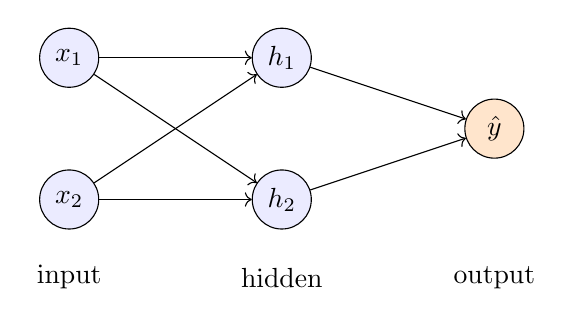
\begin{tikzpicture}[scale=0.9,neuron/.style={circle,draw,minimum size=0.75cm,inner sep=0pt,fill=blue!8}]
\foreach \i/\y in {1/1,2/-1} {\node[neuron] (x\i) at (0,\y) {$x_\i$};}
\foreach \i/\y in {1/1,2/-1} {\node[neuron] (h\i) at (3,\y) {$h_\i$};}
\node[neuron,fill=orange!20] (o) at (6,0) {$\hat y$};
\foreach \i in {1,2} \foreach \j in {1,2} \draw[->] (x\i)--(h\j);
\foreach \j in {1,2} \draw[->] (h\j)--(o);
\node at (0,-2.1) {input}; \node at (3,-2.1) {hidden}; \node at (6,-2.1) {output};
\end{tikzpicture}
\end{center}

\begin{example}[XOR with two ReLU hidden units]
Hidden: $h_1=\text{ReLU}(x_1+x_2)$, $h_2=\text{ReLU}(x_1+x_2-1)$; output $\hat y=h_1-2h_2$. Check: $(0,0)\to0$; $(0,1)\to h=(1,0)\to1$; $(1,0)\to1$; $(1,1)\to h=(2,1)\to2-2=0$. XOR solved, which no single perceptron can do.
\end{example}

\subsection{Forward pass and backpropagation (worked, numbers verified)}
\begin{story}[Passing the blame backwards]
After the committee gives a wrong answer, Somu traces \emph{who contributed how much to the error}, starting from the last layer and moving backwards, using the chain rule. Each weight is nudged in the direction that reduces the error.
\end{story}
\begin{formula}[Backpropagation recipe (sigmoid units, squared loss $L=\frac12(\hat y-t)^2$)]
Forward: $\mathbf z_1=W_1\bx+\mathbf b_1,\ \bh=\sigma(\mathbf z_1),\ z_2=\mathbf w_2^\top\bh+b_2,\ \hat y=\sigma(z_2)$.\\
Backward: $\delta_2=(\hat y-t)\,\hat y(1-\hat y)$; $\ \partial L/\partial\mathbf w_2=\delta_2\,\bh$, $\ \partial L/\partial b_2=\delta_2$;\\
$\boldsymbol\delta_1=(\mathbf w_2\,\delta_2)\odot\bh\odot(1-\bh)$; $\ \partial L/\partial W_1=\boldsymbol\delta_1\bx^\top$, $\ \partial L/\partial\mathbf b_1=\boldsymbol\delta_1$.\\
Update: $\theta\leftarrow\theta-\eta\,\partial L/\partial\theta$ (stochastic gradient descent on mini-batches).
\end{formula}
\begin{example}[A $2\!-\!2\!-\!1$ network]
Input $\bx=(1,0)$, target $t=1$; $W_1=\begin{pmatrix}0.5&-0.5\\0.3&0.8\end{pmatrix}$, $\mathbf b_1=(0.1,-0.2)$, $\mathbf w_2=(0.6,-0.4)$, $b_2=0.05$.
\begin{itemize}[noitemsep]
\item Forward: $\mathbf z_1=(0.6,0.1)$, $\bh=(0.6457,0.5250)$, $z_2=0.2274$, $\hat y=0.5566$, loss $=\frac12(0.5566-1)^2=0.0983$.
\item Backward: $\delta_2=(0.5566-1)(0.5566)(0.4434)=-0.1094$; $\partial L/\partial\mathbf w_2=(-0.0707,-0.0574)$; $\boldsymbol\delta_1=(-0.0150,\ 0.0109)$; $\partial L/\partial W_1=\boldsymbol\delta_1\bx^\top$ has first column $(-0.0150,0.0109)$ and second column $0$ (because $x_2=0$).
\item Check: a numerical derivative of the loss with respect to $W_1[1,1]$ gives $-0.015021$, equal to the backprop value.
\item After one update with $\eta=0.5$: $\hat y=0.5801$ and loss $=0.0882$ (down from $0.0983$).
\end{itemize}
\end{example}
\begin{trap}
(1) Sigmoid/tanh saturate, so gradients can vanish in deep networks (ReLU helps). (2) Never initialise all weights equally (symmetry: every neuron in a layer would learn the same thing). (3) Biases are parameters too. (4) Gradient descent finds a \emph{local} minimum; the neural-network loss is non-convex. (5) A deeper network overfits easily: use regularisation (weight decay, dropout, early stopping).
\end{trap}
% =====================================================================
\section{Model Evaluation: Bias--Variance and Cross-validation}

\begin{story}[Two bad students]
Before an exam Ramu studies only the chapter titles: he scores badly on practice tests \emph{and} on the real exam (\textbf{underfitting}). Somu memorises last year's paper word for word: he scores $100\%$ on that paper but fails when the questions change slightly (\textbf{overfitting}). ``A good student understands the pattern,'' says Somu, ``neither too simple nor too memorised. And the practice must come from questions you have \emph{not already seen}.''
\end{story}

\subsection{Underfitting, overfitting and the bias--variance decomposition}
\begin{formula}[Decomposition of expected squared error]
Suppose $y=f(x)+\varepsilon$ with noise $\E[\varepsilon]=0$, $\operatorname{Var}(\varepsilon)=\sigma^2$, and let $\hat f$ be a model trained on a random training set. At a point $x$:
\[\E\bigl[(y-\hat f(x))^2\bigr]=\underbrace{\bigl(\E[\hat f(x)]-f(x)\bigr)^2}_{\text{bias}^2}+\underbrace{\operatorname{Var}\bigl(\hat f(x)\bigr)}_{\text{variance}}+\underbrace{\sigma^2}_{\text{irreducible noise}}.\]
\begin{itemize}[noitemsep]
\item \textbf{Bias}: error from wrong assumptions (a line fitted to a curve). Simple models: high bias.
\item \textbf{Variance}: how much $\hat f$ changes if the training set changes. Flexible models: high variance.
\item \textbf{Noise} $\sigma^2$ cannot be reduced by any model.
\end{itemize}
Training error falls steadily as flexibility grows; \emph{test} error falls, then rises (U-shape). The best model sits at the bottom of the U.
\end{formula}
\begin{center}
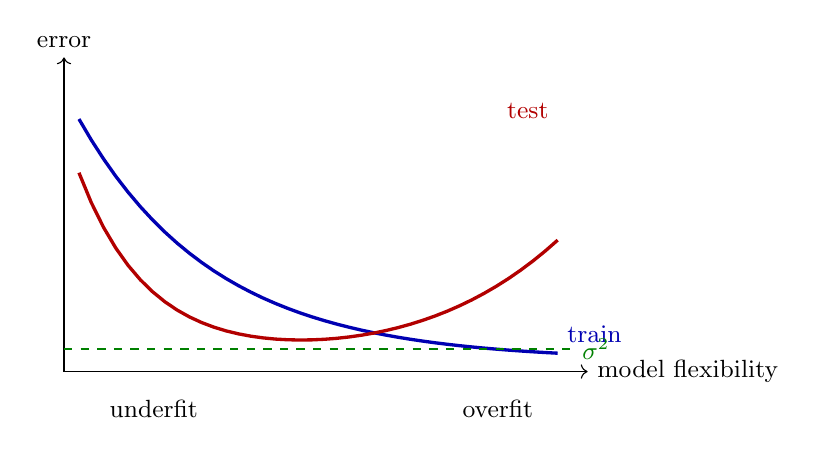
\begin{tikzpicture}[scale=0.95]
\draw[->] (0,0)--(7,0) node[right]{\small model flexibility}; \draw[->] (0,0)--(0,4.2) node[above]{\small error};
\draw[very thick,blue!70!black,domain=0.2:6.6,samples=40] plot (\x,{3.6*exp(-0.55*\x)+0.15});
\draw[very thick,red!70!black,domain=0.2:6.6,samples=40] plot (\x,{0.25+0.0008*\x^4+3.0*exp(-1.1*\x)});
\draw[thick,green!50!black,dashed] (0,0.3)--(6.8,0.3);
\node[blue!70!black,right] at (6.6,0.5) {\small train};
\node[red!70!black,above] at (6.2,3.25) {\small test};
\node[green!50!black,right] at (6.8,0.3) {\small $\sigma^2$};
\node at (1.2,-0.5) {\small underfit}; \node at (5.8,-0.5) {\small overfit};
\end{tikzpicture}
\end{center}
\begin{example}[Polynomial fits to $y=\sin2\pi x+\text{noise}$ ($\sigma=0.25$), $12$ training points, simulated]
\begin{center}
\begin{tabular}{lccc}
\toprule
degree & train MSE & test MSE & diagnosis\\
\midrule
1 & 0.145 & 0.544 & underfit: high bias (both errors high)\\
3 & 0.026 & 0.101 & good fit\\
9 & 0.006 & 1.427 & overfit: high variance (train tiny, test huge)\\
\bottomrule
\end{tabular}
\end{center}
The noise floor is $\sigma^2=0.0625$, so a test MSE of about $0.10$ for degree $3$ is close to the best possible. The degree-$9$ curve wiggles through every training point and is wildly wrong between them.
\end{example}
\begin{formula}[How the knobs move bias and variance]
\begin{center}
\small
\begin{tabular}{lcc}
\toprule
\textbf{Change} & \textbf{Bias} & \textbf{Variance}\\
\midrule
more model flexibility (polynomial degree, tree depth, network size) & $\downarrow$ & $\uparrow$\\
larger ridge/lasso $\lambda$ & $\uparrow$ & $\downarrow$\\
larger $k$ in kNN & $\uparrow$ & $\downarrow$\\
larger SVM $C$ & $\downarrow$ & $\uparrow$\\
more training data & unchanged & $\downarrow$\\
ensembling (bagging) & about same & $\downarrow$\\
\bottomrule
\end{tabular}
\end{center}
\textbf{Diagnosis:} high train error and high test error $\Rightarrow$ bias problem (use a richer model). Low train error but high test error $\Rightarrow$ variance problem (regularise, simplify, or get more data).
\end{formula}

\subsection{Train/validation/test and cross-validation}
\begin{story}[Honest practice tests]
Somu must pick the best $k$ for kNN. If he checks every $k$ on the same data he will end up fooling himself. So he sets aside a \textbf{validation set} for choosing hyperparameters and a final \textbf{test set} touched only once at the end. But when data are scarce, wasting a big chunk on validation hurts. \textbf{Cross-validation} lets every example serve as validation data exactly once.
\end{story}
\begin{formula}[$k$-fold cross-validation]
Split the data randomly into $k$ equal \textbf{folds}. For $i=1..k$: train on the other $k-1$ folds, evaluate on fold $i$. Report the \textbf{average} of the $k$ scores. With $n=100$ and $k=5$: each model trains on $80$ and is validated on $20$; $5$ models are trained. Typical $k=5$ or $10$. \textbf{Stratified} $k$-fold keeps the class proportions in every fold.
\end{formula}
\begin{formula}[Leave-one-out cross-validation (LOOCV)]
The special case $k=n$: each fold is a single example; train $n$ models, each on $n-1$ points. Nearly unbiased estimate of generalisation error, but expensive ($n$ fits) and the estimate can have high variance. For linear regression there is a shortcut (no refitting): $\text{LOO error}_i=\frac{e_i}{1-h_{ii}}$ where $h_{ii}$ is the leverage.
\end{formula}
\begin{example}[LOOCV by hand]
Data $y=\{2,4,6,8\}$; the ``model'' predicts the mean of the training points. Leave out $2$: predict $\frac{4+6+8}{3}=6$, error $(2-6)^2=16$. Leave out $4$: predict $5.333$, error $1.778$. Leave out $6$: predict $4.667$, error $1.778$. Leave out $8$: predict $4$, error $16$. LOOCV MSE $=\frac{16+1.778+1.778+16}{4}=\mathbf{8.889}$.
\end{example}
\begin{formula}[Rules of the road]
(1) Fit \emph{everything} (scaling, feature selection, imputation) inside each training fold; otherwise information leaks from the validation fold. (2) Use the test set once. (3) Larger $k$: less biased estimate, more computation, higher variance (LOOCV is the extreme). (4) \textbf{Nested} cross-validation (inner loop for hyperparameters, outer loop for the estimate) gives an honest score. (5) For time series use forward-chaining splits, not random folds.
\end{formula}
\begin{trap}
(1) Training error is a poor estimate of test error. (2) LOOCV trains $n$ models, $k$-fold trains $k$. (3) CV estimates performance; the final model is then retrained on all the data. (4) More data reduces variance, not bias. (5) Do not tune hyperparameters on the test set.
\end{trap}

% =====================================================================
\section{Clustering}

\begin{story}[Sorting a fruit market]
In a market, Ramu sees a heap of mixed fruit, with no labels. Somu groups them by looking: round and red together, long and yellow together. Nobody told him the names; he used \emph{similarity}. That is \textbf{clustering}: find groups so that points in a group are close to each other and far from other groups.
\end{story}

\subsection{$k$-means}
\begin{formula}[Lloyd's algorithm]
Choose $k$. Initialise $k$ centroids. Repeat until nothing changes: \textbf{(1) Assignment:} put each point in the cluster of its nearest centroid. \textbf{(2) Update:} move each centroid to the mean of its cluster. It minimises the \textbf{within-cluster sum of squares} $\text{WCSS}=\sum_{j=1}^k\sum_{\bx\in C_j}\norm{\bx-\mu_j}^2$; each step cannot increase WCSS, so the algorithm always \textbf{converges}, but only to a \emph{local} minimum that depends on the initial centroids (use \textbf{$k$-means++} or several restarts). Cost per iteration $O(nkd)$.\\
Weaknesses: must choose $k$ (elbow method on WCSS, silhouette score), assumes roughly round, similar-size clusters, sensitive to outliers and scale; the mean is not a data point.
\end{formula}
\begin{example}[1-D data $\{2,3,4,10,11,12\}$, $k=2$, initial centroids $3$ and $4$]
\begin{center}
\small
\begin{tabular}{c|c|c|c}
\toprule
iteration & centroids & assignment & new centroids\\
\midrule
1 & $(3,\,4)$ & $\{2,3\}\to c_1$; $\{4,10,11,12\}\to c_2$ & $(2.5,\ 9.25)$\\
2 & $(2.5,\,9.25)$ & $\{2,3,4\}\to c_1$; $\{10,11,12\}\to c_2$ & $(3,\ 11)$\\
3 & $(3,\,11)$ & same assignment & $(3,\ 11)$: \textbf{converged}\\
\bottomrule
\end{tabular}
\end{center}
Final clusters $\{2,3,4\}$ and $\{10,11,12\}$; $\text{WCSS}=(1+0+1)+(1+0+1)=\mathbf4$. Note that the point $4$ is nearer to $c_2=4$ at first, then switches to cluster $1$ when the centroids move.
\end{example}

\subsection{$k$-medoids}
\begin{formula}[$k$-medoids (PAM)]
Like $k$-means, but each cluster centre is an \emph{actual data point} (a \textbf{medoid}), and the cost is the sum of dissimilarities (any distance, often Manhattan). Swap a medoid with a non-medoid if it lowers the total cost. More robust to outliers and works with arbitrary distance matrices, but slower ($O(k(n-k)^2)$ per iteration).
\end{formula}
\begin{example}[Points $\{1,2,3,10,11\}$, $k=2$]
Medoids $\{2,10\}$: cost $|1-2|+0+|3-2|+0+|11-10|=\mathbf3$. Medoids $\{1,11\}$: $0+1+2+1+0=4$. The first choice is better, and the centres $2$ and $10$ are real data points (a mean such as $2.0$ and $10.5$ would not be).
\end{example}

\subsection{Hierarchical clustering}
\begin{story}[A family tree of points]
Somu doesn't fix the number of groups. He starts with every point alone and keeps merging the two closest groups, recording the distance at each merge. The record is a \textbf{dendrogram}; cutting it at any height gives a clustering.
\end{story}
\begin{formula}[Agglomerative (bottom-up) vs divisive (top-down)]
\textbf{Agglomerative}: start with $n$ singletons, merge the closest pair of clusters repeatedly ($n-1$ merges) until one cluster remains. \textbf{Divisive}: start with one cluster and split recursively. The distance between clusters $A$ and $B$ defines the \textbf{linkage}:
\begin{itemize}[noitemsep]
\item \textbf{Single}: $\min_{a\in A,b\in B}d(a,b)$ (nearest pair). Can produce long ``chains''.
\item \textbf{Complete}: $\max_{a\in A,b\in B}d(a,b)$ (farthest pair). Compact clusters.
\item \textbf{Average}: mean of all $|A||B|$ pairwise distances.
\item (Centroid and Ward linkage also exist.)
\end{itemize}
Naive agglomerative clustering costs $O(n^3)$ time (with a priority queue $O(n^2\log n)$) and $O(n^2)$ memory.
\end{formula}
\begin{example}[1-D points $1,2,6,8,15$]
First merges: $\{1,2\}$ at distance $1$, then $\{6,8\}$ at $2$ (all linkages agree). Then $\{1,2\}$ with $\{6,8\}$: single $=\min(5,7,4,6)=\mathbf4$; complete $=\max=\mathbf7$; average $=\frac{5+7+4+6}{4}=\mathbf{5.5}$. The point $15$ joins last:
\begin{center}
\small
\begin{tabular}{lcccc}
\toprule
linkage & merge 1 & merge 2 & merge 3 & merge 4\\
\midrule
single & 1 & 2 & 4 & 7\\
complete & 1 & 2 & 7 & 14\\
average & 1 & 2 & 5.5 & 10.75\\
\bottomrule
\end{tabular}
\end{center}
(Single: $15$ to the nearest point $8$ is $7$. Complete: $15$ to the farthest point $1$ is $14$. Average: $\frac{14+13+9+7}{4}=10.75$.)
\end{example}
\begin{center}
\begin{tikzpicture}[scale=0.75]
\draw (0,0)--(0,1)--(1,1)--(1,0); \draw (2,0)--(2,2)--(3,2)--(3,0);
\draw (0.5,1)--(0.5,4)--(2.5,4)--(2.5,2); \draw (4,0)--(4,7)--(1.5,7)--(1.5,4);
\foreach \x/\l in {0/1,1/2,2/6,3/8,4/15} \node[below] at (\x,0) {\small\l};
\draw[->] (-0.9,0)--(-0.9,7.4) node[above]{\small height}; \foreach \h in {1,2,4,7} \draw (-1,\h)--(-0.8,\h) node[left]{\small\h};
\node[right] at (5,3.5) {\small single-linkage dendrogram};
\draw[red!70!black,dashed] (-0.5,3)--(4.6,3) node[right]{\small cut at 3: 3 clusters};
\end{tikzpicture}
\end{center}
\begin{trap}
(1) $k$-means converges but not necessarily to the global optimum. (2) $k$-means uses \emph{means}; $k$-medoids uses real points. (3) Single linkage uses the \emph{minimum} distance, complete the \emph{maximum}. (4) Hierarchical clustering is deterministic (no random start) but cannot undo a merge. (5) Always standardise features before clustering. (6) Clustering has no ``accuracy'' without labels: use WCSS, silhouette, or domain judgement.
\end{trap}

% =====================================================================
\section{Principal Component Analysis (PCA)}

\begin{story}[Finding the best camera angle]
Somu photographs a long, thin table. From the end, the photo shows a tiny dot (almost all information lost). From above, the full length shows up. \textbf{PCA} finds the best viewpoint: the direction along which the data \emph{vary the most}, then the next best direction at right angles, and so on. Keep the first few directions and you compress the data while losing as little variation as possible.
\end{story}
\begin{formula}[PCA algorithm]
\begin{enumerate}[noitemsep]
\item \textbf{Centre} the data (subtract the mean of each feature; standardise too if the scales differ).
\item Compute the \textbf{covariance matrix} $C=\frac1{n-1}X_c^\top X_c$ (a $d\times d$ symmetric positive semi-definite matrix).
\item Find its \textbf{eigenvalues} $\lambda_1\ge\lambda_2\ge\dots\ge\lambda_d\ge0$ and orthonormal \textbf{eigenvectors} $\mathbf v_1,\dots,\mathbf v_d$. The eigenvectors are the \textbf{principal components (PC)} directions; $\lambda_j$ is the variance along $\mathbf v_j$.
\item Keep the top $m$; project: $Z=X_c\,V_m$ (the scores).
\end{enumerate}
\textbf{Facts:} $\sum_j\lambda_j=\operatorname{tr}(C)=$ total variance. Explained variance ratio of PC$_j$ $=\lambda_j/\sum\lambda$. Components are orthogonal and the projected scores are \emph{uncorrelated}. PCA minimises the squared reconstruction error among all $m$-dimensional linear projections. Via the \textbf{SVD} $X_c=U\Sigma V^\top$: the columns of $V$ are the PCs and $\lambda_j=\sigma_j^2/(n-1)$. PCA is unsupervised and linear; it does not use labels.
\end{formula}
\begin{example}[A $2\times2$ covariance matrix]
$C=\begin{pmatrix}2&1\\1&2\end{pmatrix}$: characteristic equation $(2-\lambda)^2-1=0\Rightarrow\lambda=3,\,1$. Eigenvectors: $\lambda=3\to\frac1{\sqrt2}(1,1)$ and $\lambda=1\to\frac1{\sqrt2}(1,-1)$. Total variance $=4=3+1$; PC1 explains $\frac34=\mathbf{75\%}$ and PC2 $25\%$. Keeping only PC1 means projecting each point on the diagonal line $y=x$.
\end{example}
\begin{example}[Ten 2-D points, computed by software]
$x=2.5,0.5,2.2,1.9,3.1,2.3,2.0,1.0,1.5,1.1$ and $y=2.4,0.7,2.9,2.2,3.0,2.7,1.6,1.1,1.6,0.9$.\\
Means $(1.81,\,1.91)$. Covariance $C=\begin{pmatrix}0.6166&0.6154\\0.6154&0.7166\end{pmatrix}$. Eigenvalues $\lambda_1=1.284$, $\lambda_2=0.0491$. First component (unit vector) $\mathbf v_1=(0.678,\,0.735)$. Explained variance: PC1 $=\frac{1.284}{1.333}=\mathbf{96.3\%}$, PC2 $=3.7\%$. The SVD singular values are $3.399$ and $0.665$ and $\frac{3.399^2}{9}=1.284$ confirms the link. Reducing from $2$ numbers to $1$ keeps $96\%$ of the variance. (The sign of a PC is arbitrary.)
\end{example}
\begin{formula}[How many components?]
Keep enough to reach a target cumulative explained variance (for example $90$--$95\%$), or look for the \textbf{elbow} in the scree plot of eigenvalues, or use cross-validation on a downstream task. With $d$ features and $n$ samples there are at most $\min(n-1,d)$ non-zero eigenvalues.
\end{formula}
\begin{trap}
(1) Centre the data first; standardise when features have different units. (2) PCA directions maximise \emph{variance}, which need not be the directions that separate classes (LDA does that). (3) Eigenvalues are variances, not standard deviations. (4) PCs are orthogonal. (5) The sum of the eigenvalues equals the trace of $C$. (6) Using fewer components always loses some variance unless the rest are exactly zero.
\end{trap}

% =====================================================================
\section{One-page Cheat Sheet}
\begin{formula}[Supervised methods]
Linear regression: $\beta_1=S_{xy}/S_{xx}$, $\beta_0=\bar y-\beta_1\bar x$, $R^2=1-\text{SSE}/\text{SST}$; normal equation $\hat{\bw}=(X^\top X)^{-1}X^\top y$; ridge $(X^\top X+\lambda I)^{-1}X^\top y$. Logistic: $p=\sigma(\bw^\top\bx+b)$, gradient $(p-y)\bx$, linear boundary. kNN: small $k$ high variance. Naive Bayes: $\argmax P(C)\prod P(x_j|C)$ with Laplace smoothing. LDA: shared $\Sigma$, linear boundary. Tree: $H=-\sum p\log_2p$, $\text{IG}=H(S)-\sum\frac{|S_v|}{|S|}H(S_v)$, Gini $=1-\sum p^2$. SVM: margin $2/\norm{\bw}$, support vectors, kernels; large $C$ $\Rightarrow$ narrow margin. NN: $\hat y=\phi(W\bx+b)$ layer by layer; params $=n_{in}n_{out}+n_{out}$; backprop uses the chain rule.
\end{formula}
\begin{formula}[Evaluation]
$\text{error}=\text{bias}^2+\text{variance}+\sigma^2$. Underfit: both errors high. Overfit: train low, test high. $k$-fold: $k$ fits, train on $\frac{k-1}{k}$ of data. LOOCV: $k=n$. Precision $=\frac{TP}{TP+FP}$, recall $=\frac{TP}{TP+FN}$, $F_1$ harmonic mean.
\end{formula}
\begin{formula}[Unsupervised]
$k$-means: assign to nearest centroid, update to cluster mean; minimises WCSS; local optimum. $k$-medoids: centres are data points. Linkage: single $=\min$, complete $=\max$, average $=$ mean pairwise distance. PCA: eigenvectors of the covariance matrix; variance ratio $\lambda_j/\sum\lambda$; $\sum\lambda=\operatorname{tr}C$; $\lambda_j=\sigma_j^2/(n-1)$.
\end{formula}

% =====================================================================
\section{Practice Questions (with answers)}
Try each one yourself first. All numeric answers were computed by code.
\begin{enumerate}[leftmargin=*,itemsep=4pt]
\item For $x=1,2,3,4,5$ and $y=2,4,5,4,5$, find the least-squares line and $R^2$. \textbf{Answer: $\hat y=2.2+0.6x$; $R^2=0.6$.}
\item Prediction of that line at $x=6$? \textbf{Answer: $5.8$.}
\item Slope after ridge regularisation with $\lambda=5$ on the same data (intercept unpenalised)? \textbf{Answer: $\dfrac{6}{10+5}=0.4$.}
\item As $\lambda\to\infty$ in ridge regression, the weights tend to? \textbf{Answer: $0$} (bias rises, variance falls).
\item Logistic regression with $\bw=(0.5,-0.25)$, $b=0.5$, $\bx=(2,4)$: probability of class $1$? \textbf{Answer: $\sigma(0.5)=0.6225$.}
\item Cross-entropy loss of that prediction if the true label is $1$? \textbf{Answer: $-\ln0.6225=0.474$.}
\item Is the decision boundary of logistic regression linear? \textbf{Answer: Yes} ($\bw^\top\bx+b=0$).
\item kNN with $k=1$: training error? \textbf{Answer: $0$} (each point is its own nearest neighbour); high variance.
\item Naive Bayes: spam score $0.5\cdot\frac35\cdot\frac35$ and ham score $0.5\cdot\frac25\cdot\frac15$ (Laplace). Posterior of spam? \textbf{Answer: $0.18/0.22=0.818$.}
\item LDA with $\mu_1=2,\mu_2=6,\sigma^2=4$, equal priors: decision boundary? \textbf{Answer: $x=4$.}
\item Entropy of a node with class counts $(1,3)$? \textbf{Answer: $0.8113$ bits.}
\item Entropy of a pure node? \textbf{Answer: $0$.}
\item $S$ has $9$ positive and $5$ negative examples. $H(S)$? \textbf{Answer: $0.940$.}
\item Information gain of Outlook with branches $(2,3),(4,0),(3,2)$? \textbf{Answer: $0.247$.}
\item Gini index of $(9,5)$? \textbf{Answer: $0.459$.}
\item SVM with $\bw=(0.4,0.4)$: margin width? \textbf{Answer: $2/\norm{\bw}=2/0.566=3.54$.}
\item Which training points determine an SVM boundary? \textbf{Answer: only the support vectors.}
\item Can a linear SVM separate XOR? A degree-2 polynomial kernel? \textbf{Answer: No; yes.}
\item Number of parameters in a $4\!-\!5\!-\!3$ feed-forward network (with biases)? \textbf{Answer: $43$.}
\item A single perceptron can learn which of AND, OR, XOR? \textbf{Answer: AND and OR, not XOR.}
\item Maximum value of $\sigma'(z)$? \textbf{Answer: $0.25$ (at $z=0$).}
\item Softmax of $(2,1,0.1)$: largest probability? \textbf{Answer: $0.659$.}
\item Network with a linear activation in every layer is equivalent to? \textbf{Answer: a single linear model.}
\item Train error $0.01$, test error $0.90$. Diagnosis? \textbf{Answer: overfitting (high variance).}
\item Both train and test errors are high. Diagnosis? \textbf{Answer: underfitting (high bias).}
\item $5$-fold CV on $100$ examples: training-set size per fold and number of models fitted? \textbf{Answer: $80$ examples; $5$ models.}
\item LOOCV on $n$ examples: number of models trained? \textbf{Answer: $n$.}
\item LOOCV MSE for $y=\{2,4,6,8\}$ using the mean of the rest as the prediction? \textbf{Answer: $8.889$.}
\item Precision, recall and $F_1$ for $TP=40,FP=10,FN=20,TN=30$? \textbf{Answer: $0.80,\ 0.667,\ 0.727$.}
\item $k$-means on $\{2,3,4,10,11,12\}$ from centroids $3$ and $4$: final centroids and WCSS? \textbf{Answer: $3$ and $11$; WCSS $=4$.}
\item $k$-medoids cost of medoids $\{2,10\}$ for points $\{1,2,3,10,11\}$ (Manhattan)? \textbf{Answer: $3$.}
\item Single, complete and average linkage distances between $\{1,2\}$ and $\{6,8\}$? \textbf{Answer: $4,\ 7,\ 5.5$.}
\item Number of merges to build a full dendrogram of $n$ points? \textbf{Answer: $n-1$.}
\item $C=\begin{pmatrix}2&1\\1&2\end{pmatrix}$: eigenvalues and variance explained by PC1? \textbf{Answer: $3,1$; $75\%$.}
\item Relationship of the SVD singular values $\sigma_j$ of the centred data matrix to PCA eigenvalues? \textbf{Answer: $\lambda_j=\sigma_j^2/(n-1)$.}
\end{enumerate}

\textbf{How to study this section:} Highest-yield for GATE DA are small numeric problems: least-squares and ridge by hand, one logistic or naive-Bayes computation, entropy/information gain, SVM margin ($2/\norm{\bw}$) and support vectors, forward pass and parameter counts of a network, bias--variance diagnosis, LOOCV and $k$-fold counts, a $k$-means iteration, linkage distances in hierarchical clustering, and eigenvalues of a $2\times2$ covariance matrix for PCA. Practise each by hand until it takes under three minutes.

\end{document}
